\begin{center}
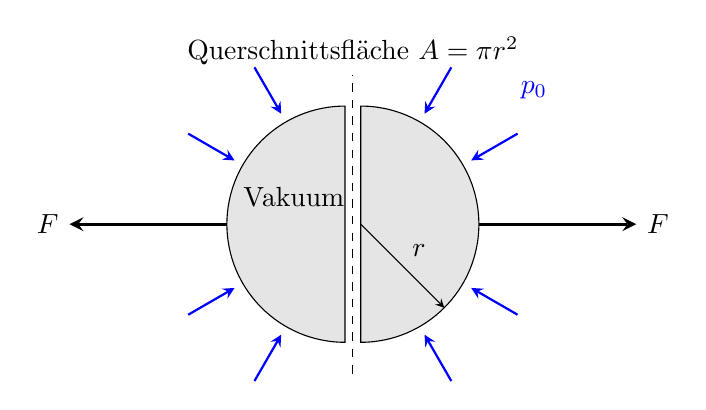
\begin{tikzpicture}[>=stealth]
 \draw[fill=gray!20] (-0.1,1.5) arc (90:270:1.5) -- cycle;
 \draw[fill=gray!20] (0.1,-1.5) arc (-90:90:1.5) -- cycle;
 \node at (-0.75,0.35) {Vakuum};
 \draw[->, very thick] (-1.6,0) -- (-3.6,0) node[left] {$F$};
 \draw[->, very thick] (1.6,0) -- (3.6,0) node[right] {$F$};
 \foreach \a in {120,150,210,240} \draw[->, blue, thick] ([shift={(-0.1,0)}]\a:2.3) -- ([shift={(-0.1,0)}]\a:1.62);
 \foreach \a in {-60,-30,30,60} \draw[->, blue, thick] ([shift={(0.1,0)}]\a:2.3) -- ([shift={(0.1,0)}]\a:1.62);
 \node[blue] at (2.3,1.7) {$p_0$};
 \draw[dashed] (0,-1.9) -- (0,1.9) node[above] {Querschnittsfläche $A = \pi r^2$};
 \draw[->] (0.1,0) -- ++(-45:1.5) node[midway, above right] {$r$};
\end{tikzpicture}
\end{center}
Die Luft drückt von aussen auf beide Halbkugeln. Die resultierende Kraft auf eine Halbkugel ist gleich gross wie die Kraft des Luftdrucks auf ihre ebene Querschnittsfläche $A = \pi r^2$, also $p_0\,\pi r^2$ (bei vollständigem Vakuum innen).

Die acht Pferde auf der einen Seite halten den acht Pferden auf der anderen Seite das Gleichgewicht; man könnte die eine Seite auch an einem Baum festbinden. Die Zugkraft zwischen den Halbkugeln ist deshalb nur
\begin{align}
 F &= \FZuF = \nPf\cdot\FPf = \FZu
\end{align}
und nicht die Kraft aller Pferde zusammen. Damit die Pferde die Kugeln (gerade) nicht trennen können, muss $p_0\,\pi r^2 \geq F$ sein. Mit dem Normdruck $p_0 = \pnmO$ ist
\begin{align}
 r &= \rmhF \\
   &= \sqrt{\frac{\nPf\cdot\FPf}{\pi\cdot\pnm}} \\
   &= \rmh \approx \result{\rmhP{-2}{2}}
\end{align}
Die Halbkugeln hatten also mindestens einen Durchmesser von etwa $\dmhP{-2}{2}$. (Guerickes Kugeln hatten tatsächlich einen Durchmesser von gut einem halben Meter; da das Vakuum nicht vollständig war, mussten sie etwas grösser sein.)
